\section*{Introdução}

A aeronave estudada neste trabalho é o Cirrus SR22, um avião ligeiro de asa baixa e com quatro a cinco lugares, fabricado pela Cirrus Aircraft (EUA). É utilizado sobretudo em viagens privadas e na formação de pilotos, e a sua estrutura é quase toda em materiais compósitos.  O SR22 é uma versão mais
potente do SR20, que realizou o primeiro voo a 21 de março de 1995. O SR22 obteve o certificado de tipo da \emph{Federal Aviation
Administration} (FAA), a autoridade de aviação civil dos EUA, a 30 de novembro de
2000, e começou a ser produzido em 2001. Na Europa, foi
certificado pela \emph{European Union Aviation Safety Agency} (EASA) a 27 de
janeiro de 2006. Segundo o fabricante, o
SR22 é a aeronave de aviação geral mais vendida do mundo todos os anos desde 2002.

Em Portugal, o SR22 é operado sobretudo por proprietários privados. Existe também um centro certificado de formação e manutenção Cirrus, a Nortávia (Maia, Porto) que dá formação de transição e recorrente a pilotos destas aeronaves e opera o SR20,
o modelo do qual o SR22 deriva. 


A forma em planta da asa apresenta-se na Figura~\ref{fig:sr22} e as principais
dimensões na Tabela~\ref{tab:sr22}. Vista de cima, a asa é mais larga na raiz do que
na ponta e tem alongamento elevado ($AR \approx 10{,}1$). Segundo o \emph{Incomplete Guide to Airfoil Usage}, a fonte recomendada na lista de
aeronaves da unidade curricular, a asa usa na raiz e na ponta um perfil Roncz,
isto é, um perfil desenhado pelo aerodinamicista John Roncz especificamente para
a Cirrus, cujas coordenadas não se encontram publicadas. O fabricante descreve a secção da
asa apenas como uma combinação de vários perfis, pelo que o perfil pode variar
ao longo da envergadura. Como indicado no enunciado, utiliza-se neste trabalho o
perfil da raiz como referência.

\begin{figure}[H]
  \centering
  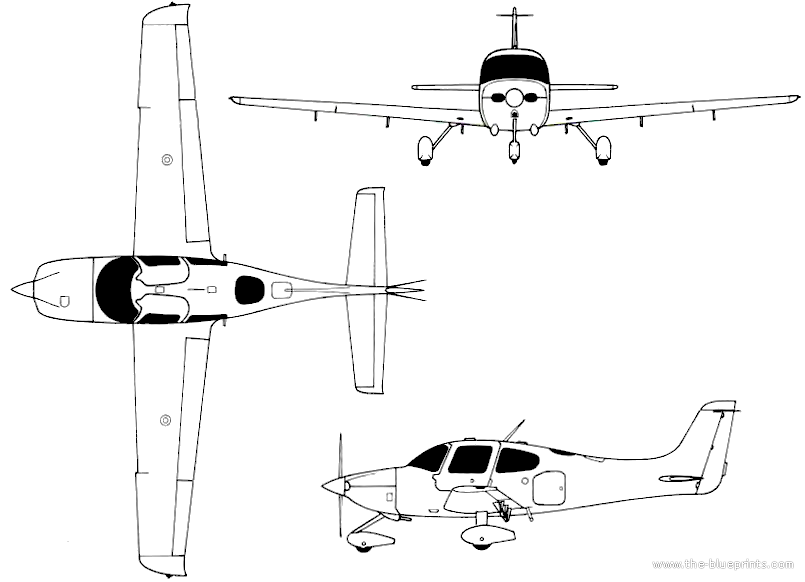
\includegraphics[width=0.4\textwidth]{imagens/blueprint.png}
  \caption{Três vistas do Cirrus SR22. Fonte: [ref].}
  \label{fig:sr22}
\end{figure}

\begin{table}[H]
  \centering
  \caption{Principais características do Cirrus SR22 (números de série 3915 e
  seguintes).}
  \label{tab:sr22}
  \begin{tabular}{lc}
    \toprule
    Parâmetro & Valor \\
    \midrule
    Envergadura $b$ [m]                         & 11,67 \\
    Área alar $S$ [m$^2$]                       & 13,46 \\
    Alongamento $AR = b^2/S$                    & 10,1 \\
    Corda na raiz / na ponta [m]                & $\approx 1{,}49$ / $0{,}89$ \\
    Enflechamento (1/4 da corda) [$^\circ$]     & $\approx 0$ \\
    Massa máxima à descolagem [kg]              & 1\,633 \\
    Velocidade de voo de referência [km/h]      & 340 \\
    Número de Mach                              & 0,28 \\
    Perfil na raiz / na ponta                   & Roncz / Roncz \\
    \bottomrule
  \end{tabular}
\end{table}

Não estando disponíveis as coordenadas do perfil do SR22, utilizou-se como perfil
de referência (raiz) o perfil Roncz/Marske-7 da base de dados de coordenadas da
UIUC, que, como o nome indica, é também um perfil associado a Roncz. As suas
principais características geométricas resumem-se na Tabela~\ref{tab:perfil}.
Destaca-se a linha média com \emph{reflex} junto ao bordo de fuga (ordenada
negativa), característica dos perfis de asa voadora.
 
\begin{table}[H]
  \centering
  \caption{Características geométricas do perfil Roncz/Marske-7.}
  \label{tab:perfil}
  \begin{tabular}{lcc}
    \toprule
    Parâmetro & Valor [\%$c$] & Posição $x/c$ \\
    \midrule
    Espessura máxima         & 12,1   & {[TODO]} \\
    Curvatura máxima         & 2,8    & {[TODO]} \\
    Ordenada mínima da linha média & $-0{,}5$ & {[TODO]} \\
    \bottomrule
  \end{tabular}
\end{table}

Para estudar este perfil consideram-se três métodos, de complexidade e custo
computacional crescentes. A teoria dos perfis delgados é um método analítico que
admite escoamento invíscido e incompressível e representa o perfil apenas pela sua
linha média, supondo espessura, curvatura e ângulo de ataque pequenos. O método
dos painéis é um método numérico, também invíscido, que discretiza o contorno real
do perfil em $N$ painéis com distribuições de vórtices, tendo assim em conta a
espessura. Por fim, a simulação CFD no OpenFOAM resolve numericamente as
equações de Navier--Stokes com um modelo de turbulência, incluindo os efeitos da
viscosidade, como a camada limite e a separação do escoamento.

A velocidade de voo de referência é $V_\infty = 340$~km/h ($\approx 94{,}4$~m/s),
a que corresponde $M_\infty \approx 0{,}28$. Como
$M_\infty < 0{,}3$, as variações de massa volúmica são pequenas e o escoamento
pode ser considerado incompressível, hipótese em que assentam a
teoria dos perfis delgados e o método dos painéis. Com os valores da atmosfera
padrão ao nível do mar ($\rho_\infty = 1{,}225$~kg/m$^3$,
$\mu_\infty = 1{,}789\times10^{-5}$~Pa\,s) e a corda na raiz, o
número de Reynolds é
\[
  Re = \frac{\rho_\infty V_\infty c_r}{\mu_\infty}
     \approx \frac{1{,}225 \times 94{,}4 \times 1{,}49}{1{,}789\times10^{-5}}
     \approx 9{,}6\times10^{6}.
\]

